\newpage
\newcommand{\myuv}[1]{\quotedblbase #1\textquotedblleft}

\chapter{Úvod}
5G je pátá generace mobilních sítí pro přenos dat. Tato technologie se v současné době již globálně instaluje a částečně se i používá. Od předchůdce (4G) se liší v násobně větší přenosové rychlosti -- v současné době je uvažována rychlost 1Gbps, ale v budoucnu (cca rok 2030) se mluví až o 20Gbps. Další klíčový parametr je nízká latence -- plánovaná latence je 1ms, zatím se reálná latence pohybuje řádově v několika milisekundách. Další důležitý milník, kterého je v plánu dosáhnout je kapacita počtu připojených zařízení -- v plánu je jeden milion zařízení na metr čtverečních \cite{QualcommUvod}.  
\section{Příklady použití}\label{uziti}
V tomto odstavci shrnu technologie, které by měl podle normy obsahovat kompletní sytém 5G a jejich následné využití/použití \cite{5Gtechnologi}.
\par
\subsubsection{eMBB (enhanced Mobile Broadband)}
Tuto technologii využívají služby, které vyžadují velké toky dat napříč internetem. Dá se například  předpokládat, že přibudou  uživatelé, kteří si budou přehrávat videa/filmy ve vysoké kvalitě a tím zvýší nároky na datový provoz. Dále se očkává masivnější využívání cloud computingu. Jedná se o službu, která provádí povětšinou složité a náročné operace vzdáleně na cloudu a výsledky posílá zpátky uživateli, uživatel tedy potřebuje jen základní hardware, který slouží na zadávání požadavků a zobrazování výsledků \cite{CloudComputing}. Názorným příkladem  je např. hraní her v cloudu, kdy hráč zadává instrukce, ty jsou přenášeny na server kde hra fyzicky běží a uživateli se zpátky posílá obraz se zvukem \cite{CloudGaming}.   
\par
\subsubsection{mMTC (massive Machine Type Communications)}
Podstata technologie spočívá ve velkém počtu malých poměrně datově nenáročných zařízeních (Internet věcí \cite{IOT}). Tyto zařízení by se mohli využít pro chytrá města či chytrá domácnost. Očekává se obrovský přírůstek těchto zařízení, proto se síť 5G dimenzuje na tyto kapacity hned od začátku \cite{UseCases}.
\par
\subsubsection{URLLC (Ultra Reliable Low Latency Communications)}
Uplatnění velmi nízké latence a velmi vysoké spolehlivosti by našli například služby autonomního řízení aut či jiných dopravních prostředků. Hovoří se i o vzdálených lékařských zákrocích, kdyby mohl doktor operovat vzdáleně pacienty z celého světa \cite{UseCases}. 

\begin{figure}[ht]
\centering
    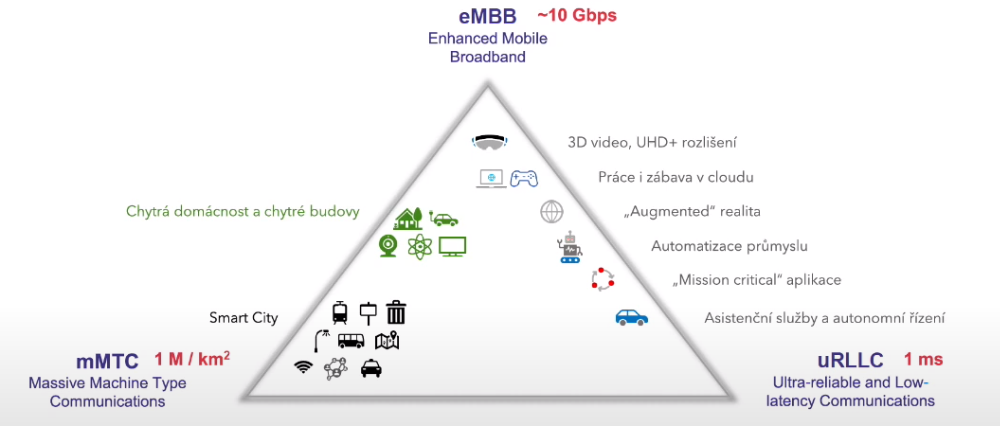
\includegraphics[width=\textwidth]{sluzby.png}
    \caption{Diagram užití technologiích použitých v 5G. Získáno z \cite{Cetin}}
   \label{fig:mods}
\end{figure}
\subsection{Vize do budoucna}
   S příchodem 5G sítí se plánují velice ambiciózní  vize. Často se tak mluví o chytrých městech, autech, silnicích atd. V případě chytrých aut se plánuje zdokonalit autonomní řízení - auta by se měla nejenom autonomně řídit, ale zároveň by měla navzájem komunikovat a sdělovat si důležité informace. Tato komunikace případně povede k lepší propustnosti silnic a k většímu bezpečí na silnici. Autonomní řízení by také hrálo velkou roli třeba v automatizaci agronomie \cite{Cetin}. 
\par
Všechny tyto vize však potřebují pevný základ v podobě stabilní, rychlé a spolehlivé sítě, která bude mít pokrytí takřka všude. Tyto podmínky se snaží 5G sítě splnit.

\chapter{Technologie}

\section{Přenosová pásma}
Na rozdíl od svého předchůdce 5G využívá pro přenos signálu velkou škálu frekvencí s různými vlnovými délkami. 
Idea je jednoduchá -- na hustě obydlené zóny budou použity krátké vlny  a na např. venkov či volné prostranství budou použity dlouhé vlny.  Tímto krokem dojde k co největšímu územnímu pokrytí \cite{Cetin}.
\par
5G bude využívat již používané frekvenční pásma mobilních sítí (2G, 3G a 4G). K těmto pásmům přibude oblast nad 700 MHz dříve okupovaná televizním signálem a nově vysokofrekvenční pásma vybraných na intervalech od 24.25 GHz do 71 GHz \cite{pasma}.

\section{Paprskování (beam forming, beam steeering) }
Jedná se o technologie, které umožňují cílit paprsky signálu přímo na uživatele. Základní princip funguje díky většímu množství antén, které signál posilují ve směru k uživateli a v ostatních směrech tento signál ruší. Tímto způsobem se zvýší možný počet připojených zařízení k přístupovému bodu a zároveň se navýší rychlost přenášení dat -- zařízení se nebudou muset dělit o stejné frekvence \cite{BeamForming}. Výhody této antény jsou však vykoupeny potřebným výpočetním výkonem pro provoz  a řádově vyšší pořizovací cenou. Tato technika se již v malém měřítku používá v některých wi-fi přístupových bodech. 
\begin{figure}[h]
\centering
   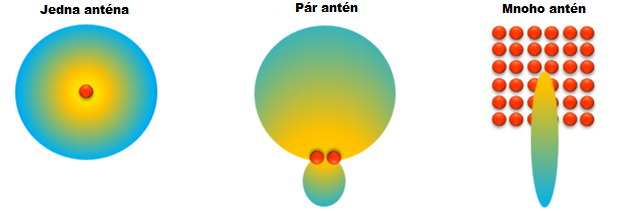
\includegraphics[width=350px]{anteny.png}
    \caption{Demonstrace paprskování za pomocí více antén. Převzato a přeloženo z \cite{BeamFormingObr}.}
    \label{fig:anteny1}
\end{figure}
\par 
\subsection{mMIMO}
Jedná se o systém vysílací jednotky využívající výše zmíněné technologie. Zkratka mMIMO znamená \myuv{masive Multiple Input Multiple Output}. Jak již význam zkratky napovídá, jedná se o systém, který může přijímat a vysílat signál k velkému množství uživatelů v reálném čase. Anténí jednotka se skládá z logických portů. V praxi se používá 32 nebo 64 těchto logických portů. Na tyto porty připadne 128/192 fyzických antén \cite{BeamForming}.
\par
Hmotnost hraje podstatnou roli u antény -- pokud přesáhne limity dané normami pro bezpečnost práce ve výškových pracovištích, musí se antény instalovat např. jeřábem, což značně zvyšuje náklady na instalaci a údržbu. Proto se použití této technologie nejvíce vyplatí  pro antény operujících na  vyšších frekvencí (pro C-band). Pro antény dlouhých vln značně rostou rozměry antény a tím i hmotnost \cite{Cetin}.  

\begin{figure}[ht]
\centering
   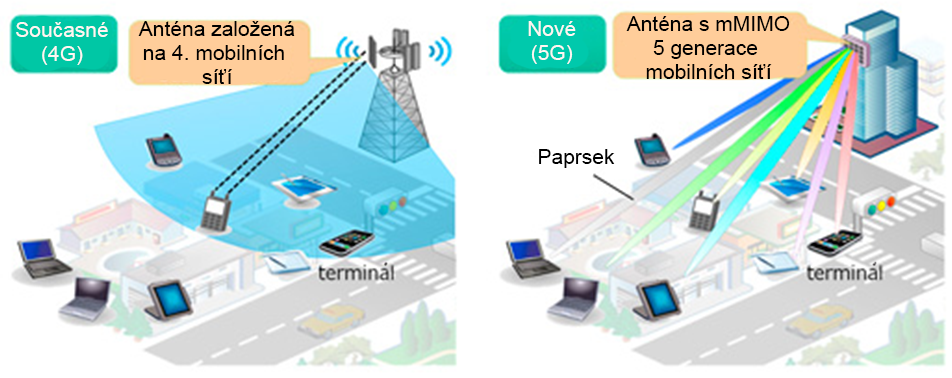
\includegraphics[width=350px]{mmimo.png}
    \caption{Na obrázku je zobrazen přenos dat na starší generací mobilní sítě v porovnání s novou. Převzato a přeloženo z \cite{mmimoObr}.}
    \label{fig:anteny2}
\end{figure}
\section{Slicing}
Jak bylo již zmíněno v sekci \myuv{příklady užití} \ref{uziti}, každá služba bude mít své specifické požadavky. Proto bude možné fyzickou síť virtuálně rozdělit do více vrstev. Každá vrstva bude obsahovat pro ni potřebné technologie. Podle potřeby se pak jednotlivým vrstvám budou přiřazovat potřebné zdroje. Každá vrstva bude moci obsahovat různé úrovně zabezpečení \cite{Slicing} -- např. síť pro monitorování počasí nebude potřebovat takovou míru bezpečnostních mechanismů jako síť určená pro provádění internetových plateb. 
\section{Infrastruktura}
Pro korektní implementaci a dodržení návrhových požadavků bude potřeba modifikovat starou architekturu sítí -- ve velkých městech bude potřeba násobně více antén/buněk než do posud, ty poté budou muset být propojeny optickými kabely, aby byly splněny požadavky na latenci a propustnost. Do budoucna je plánováno pokrytí vnitřku budov a přístup k síti i např. v letadle \cite{Cetin}.
\par


\chapter{Bezpečnost}
S postupem času se očekává mnohonásobně více zařízení připojených do sítě 5G. Velká část těchto zařízení však bude často primitivních/\myuv{hloupých} typu např.: reproduktor či senzory (technologie IOT).  Do posud byla tato zařízení \myuv{schována} za routerem či firewallem a byla do jisté míry chráněná těmito prvky. S příchodem 5G se počítá s přímým napojením na tuto síť, byť tyto zařízení nemají sofistikované zabezpečení alespoň na úrovni smartphonů/notebooků. Proto se musí zabezpečení integrovat přímo do sítě \cite{Avast}.
\section{Očekávané útoky}
V této sekci popíšu některé z očekávaných útoků na síť 5G a zařízení k ní připojených.
\subsection{Dos, DDos, Botnet}
Tyto útoky mají obvykle společný cíl -- vždy jde o úmyslné přetížení nějaké komunikace/služby velkým počtem zbytečných požadavků. Útoky Dos jsou zpravidla vedeny z jedno počítače. DDos útoky jsou prováděny z větším počtem počítačů. Botnet je označení pro síť těchto počítačů, obvykle se útočící zařízení nedostanou do této sítě vědomě -- obvykle jde o počítače napadené nějakou formou počítačového viru \cite{Ddos}. Tyto útoky však nejsou na poli internetu žádnou novinkou. 
\par
S příchodem 5G a jeho parametry -- velmi nízkou latencí, velkou přenosovou rychlostí a velkým množstvím zařízení se tyto útoky stávají ještě nebezpečnými. A fakt že přibude více zařízeních (často nijak nechráněných) připojených do této sítě situaci nijak nevylepšuje. 
\par
Řešením je včasná detekce těchto útoků a případné odklonění v reálném čase. Do tohoto procesu by měla významně přispět umělá inteligence a strojové učení, která včas rozpozná škodlivou komunikaci a odfiltruje ji \cite{DdosProtection}. Tyto mechanismy již fungují a můžete si je pronajmou formou cloudové služby -- komunikace od klientů putuje do této služby, která ji odfiltruje a přepošle směrem k vaším serverům \cite{DdosShield}. V 5G sítích se očekává implementace těchto mechanizmů přímo do sítě. 
\subsection{Vynucená degradace komunikace}
Jedná se typ útoku, kdy útočník vynutí přechod zařízení na nižší generaci sítě pomocí nějakého typu rušičky. Po tomto vynucení může útočník snáze vystopovat nebo odposlouchávat komunikaci \cite{KshetriNir20205SaY}.
\subsection{Vydávání se za obslužnou síť }
V těchto typech útoku se potencionální útočník vydává za legitimní obslužnou síť pro autentizaci uživatele a pokouší se při připojení zařízení na tento server odchytit důležitá data v průběhu ověření zařízení. Tento problém řeší ověřovací mechanizmy popisované v sekci \ref{Autentizace} .
\newpage
\section{Ověření uživatele}\label{Autentizace}
Ačkoliv většina 5G sítí zatím fungují v hybridním módu (non-standalone) -- ověření a řízení se provádí přes sítě starších generací \cite{Cetin}, tak popíšu jak probíhá autentizace uživatele v čistě 5G síti. 
\\
\\
Pozn.: Celá sekce čerpá z podkladů \cite{Schwarz}, \cite{autentizace3} a \cite{autentizace2}.
\subsection{Hlavní aktéři}
\begin{itemize}
    \item  USIM -- SIM karta s privátním šifrovacím klíčem. Nachází se v zařízení, které žádá o autentizaci. Stejný klíč je uložen i v jádru domácí sítě(UDM/ARPF)
    \item SEAF(Security Anchor Function) -- Slouží jako prostředník mezi uživatelem a domovskou sítí. 
    \item  SEPP(Security Edge Protection Proxy) -- slouží k zabezpečené komunikací mezi domovskou a obslužnou sítí.
    \item  AUSF(Authentication Server Function) -- Provádí autentizaci v domácí síti. 
   \item  SIDF(Subscription Identifier De-concealing Function) -- Získává pravou identitu SUPI ze SUCI.
    \item UDM/ARPF -- Repositář uložených klíčů. Funkce ARPF rozhoduje o autentizační metodě ověření.
\end{itemize} 
\begin{figure}[!ht]
\centering
   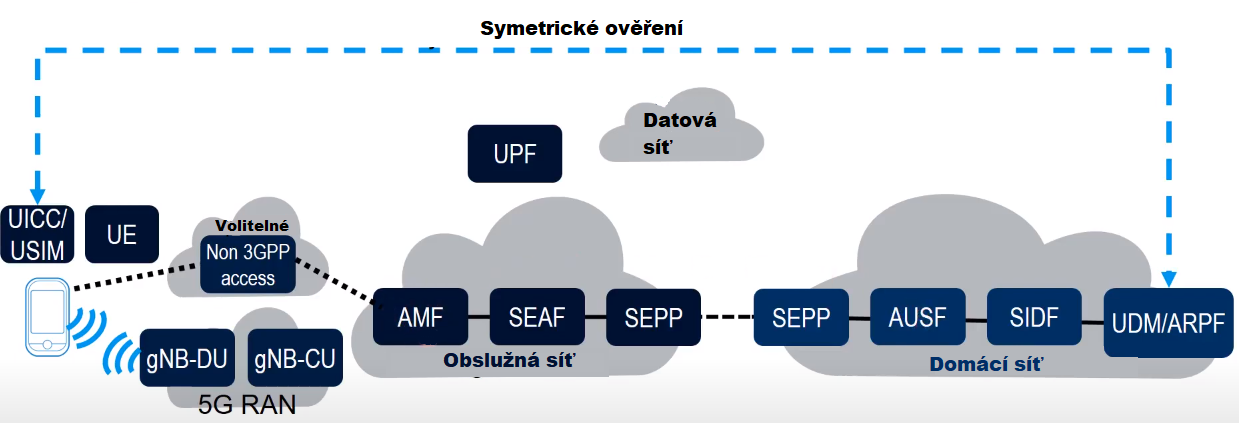
\includegraphics[width=\textwidth]{autentizace1.png}
    \caption{Obrázek zobrazující klíčové komponenty pro autentizaci uživatele. Převzato a přeloženo z \cite{Schwarz}.}
    \label{fig:autentizace1}
\end{figure}
\subsection{Autentizační zprávy}
\begin{itemize}
    \item  SUPI--permanentní identifikátor klienta, je uložen na SIM kartě klienta a v repositáři domovské sítě(UDM/ARPF). 
    \item  SUCI--zašifrované SUPI. Náhradou SUCI může být dočasný identifikátor (5G-GUTI).
    \item Autentifikační vektor\label{vector} -- vektor je generován v UDM/ARPF. Skládá se z AUTH tokenu, XRES tokenu a klíče $K_{AUSF}$.
\end{itemize} 
\newpage
\subsection{Průběh ověření}
Zařízení se může do sítě 5G připojit buď přímo přes síť 5G RAN nebo např. přes Wi-Fi router připojený k této síti (na obrázku \ref{fig:autentizace1} zobrazeno jako \myuv{Non 3GPP access}). V případě připojení  přes zařízení které není 3GPP (např. zmiňovaný Wi-Fi router) se musí navíc mezi obslužnou sítí a zařízením  vytvořit VPN tunel \cite{autentizace3}.
\par
Autentizace začíná žádostí na ověření, tato žádost obsahuje SUCI a je propagovaná až do ARPF. Pokud je v UDM/ARPF záznam o daném SUCI, tak se pomocí SIDF toto SUCI rozšifruje na SUPI. Poté UDM/ARPF vybírá metodu autentizace (5G-AKA, EAP-AKA). 5G-AKA se volí v případě, kdy se musí ověřit obslužná síť, EAP-AKA je použit v případě, kdy je zaručena integrita obslužné sítě (např. je součástí domácí sítě) \cite{Schwarz}. V situaci na popisovaném obrázku \ref{fig:autentizace2} je zvolena 5G-AKA. 
\par
Metoda 5G-AKA začíná zasláním autentizačního vektoru \ref{vector} a SUPI do AUSF. AUSF si uloží klíč $K_{AUSF}$ a spočítá HXRES. Poté zasílá token AUTH a vypočítané HXRES směrem do SEAF. SUPI se při tomto kroku neposílá, aby se zabránilo zneužití v případě zjištěné nedůvěry mezi obslužnou a domácí sítí. 
\par
SEAF si z této správy uloží HXRES a zašle do zařízení získaný token AUTH. Pomocí tajného klíče, který sdílí s domácí sítí si zařízení ověří token AUTH. Při úspěšném ověření zařízení považuje síť za autorizovanou. Po tomto ověření zasílá zařízení spočítaný RES token do SEAF. SEAF spočítá z této odpovědi HRES a porovná s uloženým záznamem. 
\par
V dalším kroku je token RES přeposlán do AUSF. Tato odpověď je porovnána s uloženým záznamem XRES. Po úspěšném ověření je vypočten  $K_{SEAF}$ a jeho derivace spolu se SUPI je odeslána zpět do SEAF. Zpráva o úspěchu je odeslána do UDM/ARPF pro účely auditu \cite{autentizace3}. 
\par
Po tomto procesu je zařízení autentizované. 
\begin{figure}[!ht]
    \centering
    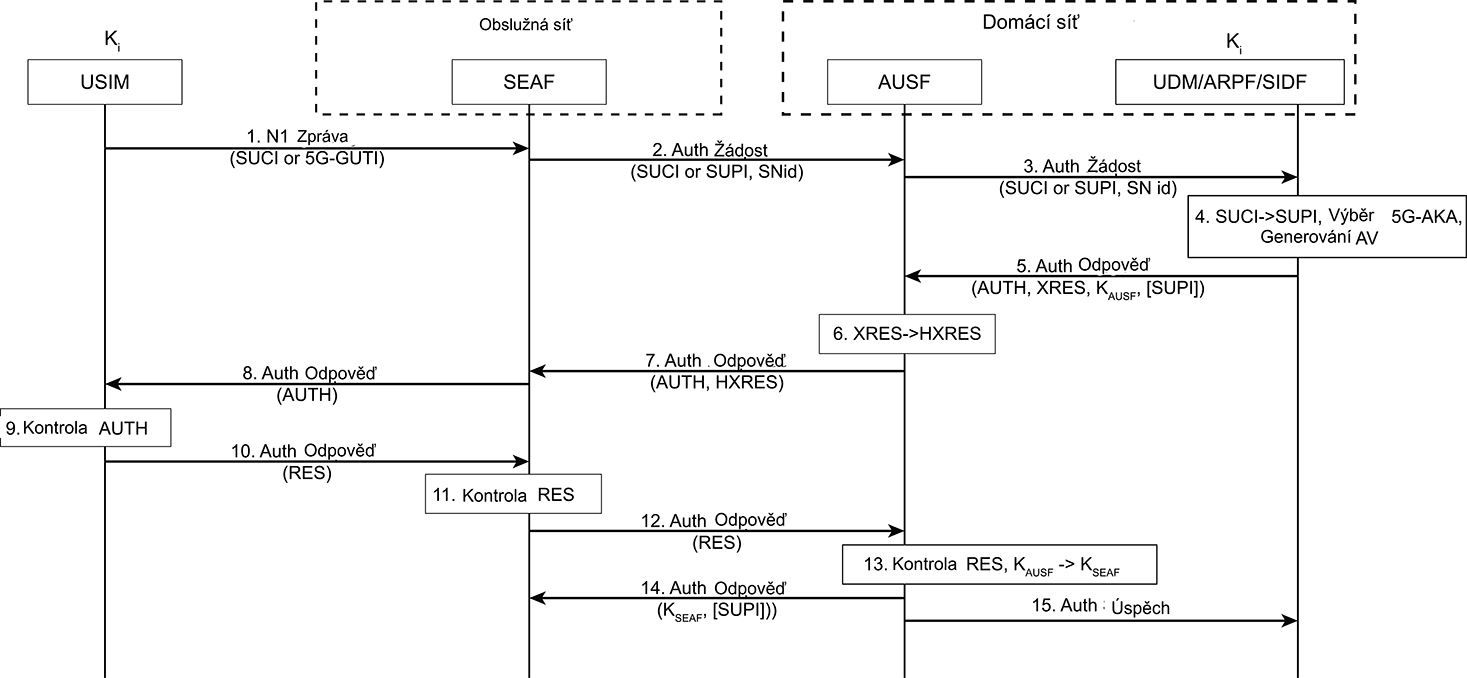
\includegraphics[width=\textwidth]{autentizace2.jpg}
    \caption{Obrázek zobrazující průběh autentizace zařízení. Převzato a přeloženo z \cite{autentizace3}.}
    \label{fig:autentizace2}
    \end{figure}
\chapter{Závěr}\label{zaver}
Sítě 5G mají velký potenciál, využívají nejmodernější techniky a  snaží se tak být co nejefektivnější.  Jejich úspěch je však  podmíněn zabezpečením této sítě. V případě úspěchu nabídnou zázemí pro širokou škálu služeb a techniky.

